%!TEX root = ../thesis.tex
%*******************************************************************************
%****************************** Third Chapter **********************************
%*******************************************************************************
\chapter{Resultados y Discusión}\label{chap:result}

\begin{graybox}
\begin{itemize}
\item El principal resultado de este trabajo es la extensión pg\_landmetrics, en la cual se ha colaborado en un importante porcentaje de funcionalidades (\textit{commits}).
\item Las métricas implementadas en forma de funciones se han validado sistemáticamente para asegurar que devuelven el resultado correcto.
\item Se ha desarrollado un caso de uso completo basado en la aplicación propuesta en (ref al mockup) con el que se han obtenido resultados prometedores (\textit{usabilidad} y volumen).
\end{itemize}
\end{graybox}

Intro a los resultados... codigo/commits y caso de uso

En la subsección \ref{sec:pglandmetrics} se describen cuantitativamente las aportaciones realizadas en este proyecto y que corresponden al grueso del presente trabajo. A continuación, en la subsección \ref{sec:caso_uso} se presentan los resultados de un caso de uso o experiencia computacional en el que se pone a prueba la extensión desarrollada. Era importante permitir que los usuarios del SIOSE calculasen métricas de una manera sencilla e intuitiva, pero también que pudiesen manejar un gran volumen de datos que en otras aplicaciones, como las citadas en el capítulo de \nameref{chap:intro}.

\section{pg\_landmetrics \label{sec:pglandmetrics}}

Cuantitativamente, detalles de mi aportación frente al total de la extensión... y para cada una un comentario o valoración personal.

\begin{figure}
\begin{center}
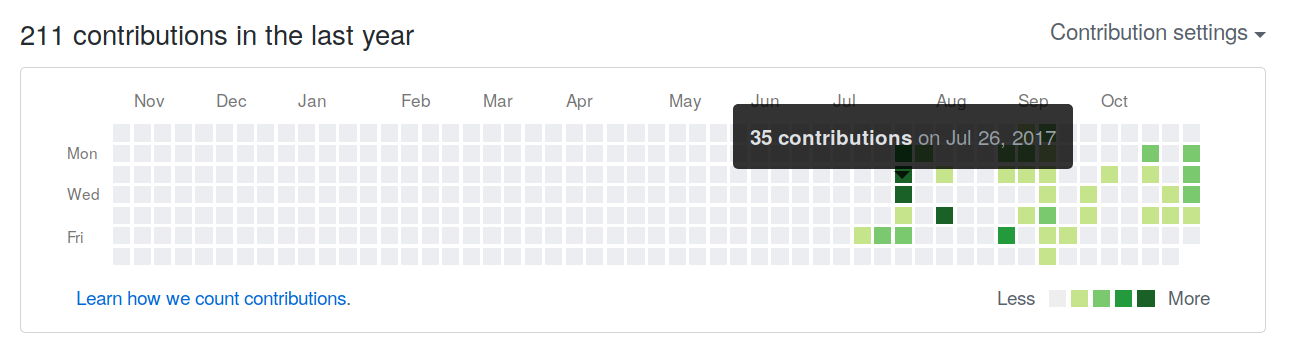
\includegraphics[width=\textwidth]{ResultadosyDiscusion/Figs/contributions.png}
\caption{Título. \label{fig:contrib}}
\end{center}
\end{figure}

\begin{figure}
\begin{center}
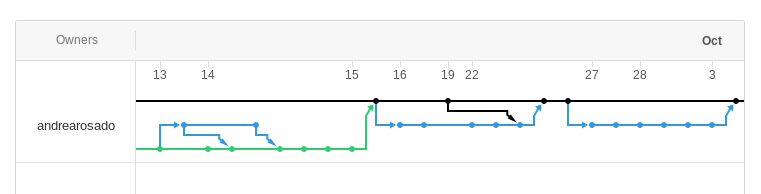
\includegraphics[width=\textwidth]{ResultadosyDiscusion/Figs/network-1.png}
\caption{Título. \label{fig:network1}}
\end{center}
\end{figure}

\begin{figure}
\begin{center}
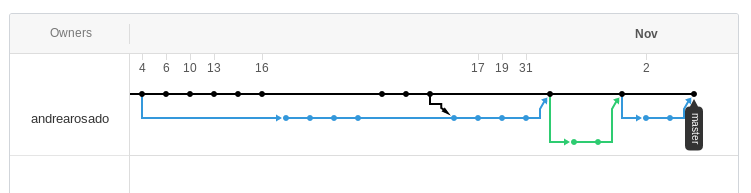
\includegraphics[width=\textwidth]{ResultadosyDiscusion/Figs/network-2.png}
\caption{Título. \label{fig:network2}}
\end{center}
\end{figure}


\section{Caso de uso sobre el SIOSE-2011 \label{sec:caso_uso}}


Listing con la consulta final, una única línea frente a las n líneas que serían necesarias en una única consulta SQL.

Figuras correlación entre dos zonas de estudio grandes...


Volumen de los datos (TABLA). La base de datos del SIOSE 2011 proporcionada por el equipo nacional del SIOSE era muy voluminosa ()



